
\item Two men are walking along a horizontal straight line in the same direction. The man in front walks at a speed \(1.0 \, \text{m s}^{-1}\) and the man behind walks at a speed \(2.0 \, \text{m s}^{-1}\). A third man is standing at a height \(12 \, \text{m}\) above the same horizontal line such that all three men are in a vertical plane. The two walking men are blowing identical whistles which emit a sound of frequency \(1430 \, \text{Hz}\). The speed of sound in air is \(330 \, \text{m s}^{-1}\). At the instant, when the moving men are \(10 \, \text{m}\) apart, the stationary man is equidistant from them. The frequency of beats in Hz, heard by the stationary man at this instant, is \underline{\hspace{3cm}}.
\begin{solution}
    \begin{center}
        \begin{tikzpicture}
            \tzcoor*(-2, 0)(A)
            \tzcoor*(2, 0)(B)
            \tzcoor*(0, 2)(C)
            \tzline(-3, 0)(3, 0)
            \tzline(0, -1)(0, 3)
            \tzline+[->](A)(1, 0){$2\mps$}[b]
            \tzline+[->](B)(1, 0){$1\mps$}[b]
            \tzline[dashed](A)(C)
            \tzline[dashed](B)(C)
            \tzline[|<->|]<-0.25, 0>(0, 0)(C){$12\m$}[ml]
            \tzline[|<->|]<0, -0.5>(A)(B){$10\m$}[mb]
        \end{tikzpicture}
    \end{center}
    \begin{align*}
        \intertext{Since the men are in the same vertical plane and equidistant from the stationary man, sound waves from both men reach the stationary man simultaneously, forming beats. The beat frequency is equal to the difference between the apparent frequencies of the whistles heard by the stationary man.}
        \intertext{For the first man (walking at $1.0 \, \text{m s}^{-1}$) away:}
        f'_1 &= f \cdot \dfrac{v}{v + v_1}\\
        \intertext{For the second man (walking at $2.0 \, \text{m s}^{-1}$) towards:}
        f'_2 &= f \cdot \dfrac{v}{v - v_2}\\
        \intertext{The frequency of beats is the difference between $f'_1$ and $f'_2$:}
        f_{\text{beats}} &= |f'_1 - f'_2|\\
        &= f \left|\dfrac{v}{v + v_1} - \dfrac{v}{v - v_2}\right|, \qquad v_1= 1\cdot \cos\theta, v_2=2\cdot \cos\theta\\
        &= 1430 \left| \dfrac{330}{330 + \frac{5}{13}} -  \dfrac{330}{330 - \frac{10}{13}}\right|\\ 
        &= 1430 \cdot \left|\dfrac{1}{1 + \frac{5}{13 \times 330}} - \dfrac{1}{1 - \frac{10}{13\times 330}}\right|\intertext{Solving the above expression using binomial expansion as the denominator is small:}
        &\approx 1430 \cdot \left|\left(1 - \dfrac{5}{13 \times 330}\right) - \left(1 + \dfrac{10}{13 \times 330}\right)\right|\\
        &= 1430 \cdot \left|\dfrac{5}{13 \times 330} + \dfrac{10}{13 \times 330}\right|\\
        &= 1430 \cdot \dfrac{15}{13 \times 330}\\
        &= 110 \cdot \dfrac{15}{330}\\
        &= 5 \, \text{Hz}.
        \intertext{Therefore, the frequency of beats heard by the stationary man is \(5 \, \text{Hz}\).}
    \end{align*}
\end{solution}